\documentclass[12pt]{article}
\usepackage{amssymb}
\usepackage[UTF8]{ctex}
\usepackage{geometry}
\usepackage{units}
\usepackage{pifont}
\geometry{
	a4paper,
	total={150mm,237mm},
	left=30mm,
	top=27mm,
	}
\usepackage{amsmath}
\usepackage{enumerate}
\usepackage{lipsum}
\usepackage{graphicx}
\usepackage{hyperref}
\usepackage{indentfirst}
\usepackage[graphicx]{realboxes}
\usepackage{booktabs}
\usepackage{cases}
\usepackage{subfig}  
\usepackage{float}

\setlength{\parindent}{2em}
\title{HW4}
\author{姓名:陈锐林,学号:21307130148}
\date{\today}

\begin{document}
\maketitle
\begin{LARGE}
    \noindent Chapter16\\
\end{LARGE}
\begin{large}
	\noindent Question1\\
\end{large}
\hspace*{2em}这题中三行命令的前面都是相同的。address space size是128,所以需要7位来标识。在7位的虚拟地址中,大于64(0x40)的是seg1,小于的是seg0。再根据界限寄存器,所以合理的虚拟地址应该在(0$\thicksim$19),(108$\thicksim$127)。\par
(1)生成的四条VA为:108/97/53/33/65,显然只有第一条是可取的,其他都是segmentation violation;再由512-20=492,得到其真实物理地址(seg1中)。\par
(2)生成的四条VA为:17/108/97/32/63,前两条是有效的,剩下三条是segmentation violation;0+17=17,512-20=492,得物理地址为17(seg0),492(seg1)。\par
(3)生成的四条VA为:122/121/7/10/106,前四条是有效的,第五条是segmentation violation;512-6=506,512-7=505,0+7=7,0+10=10,得物理地址为506(seg1),505(seg1),7(seg0),10(seg0)。\\

\begin{large}
	\noindent Question2\\
\end{large}
\hspace*{2em}这题在上面已经指出了,seg0最高有效:19,seg1最高有效:108;最低和最高非法:20/127。验证如下:
\begin{figure}[h]
    \centering
    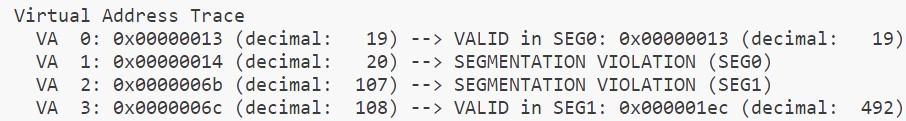
\includegraphics[width=13cm,height=3cm]{p1.jpg}
\end{figure}\\

\begin{large}
	\noindent Question3\\
\end{large}
\hspace*{2em}调用命令:python3 ./segmentation.py -a 16 -p 128 -A 0,1,2,3,4,5,6,7,8,9,10,11,12,13,14,15 --b0 0 --l0 2 --b1 16 --l1 2 -c就可以了,能得到如下结果:
\begin{figure}[h]
    \centering
    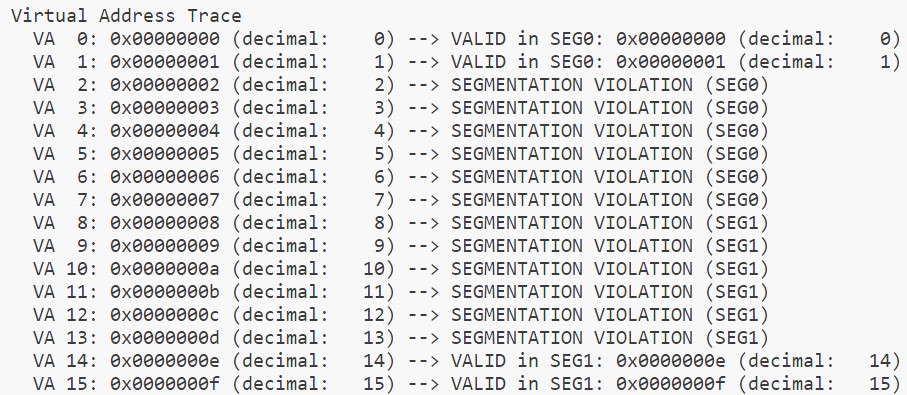
\includegraphics[width=13cm,height=7cm]{p2.jpg}
\end{figure}\\

\begin{large}
	\noindent Question4\\
\end{large}
\hspace*{2em}为了让大约90\%的地址都是有效的,借鉴3中的思路可以知道,应该满足:(limit0+limit1)/address\_space\_size $\geq$ 90\%。\\

\begin{large}
	\noindent Question5\\
\end{large}
\hspace*{2em}只要让界限长度为0,所有的VA就都无效了。\\

\begin{LARGE}
    \noindent Chapter18\\
\end{LARGE}
\begin{large}
	\noindent Question1\\
\end{large}
\hspace*{2em}根据观察,随着地址空间的增大,页表会变大;而随着页大小的增加,页表会变小。很大的页可能会导致开销增大,而且利用率会下降。\\

\begin{large}
	\noindent Question2\\
\end{large}
\hspace*{2em}对于命令:"python3 ./paging-linear-translate.py -P 1k -a 16k -p 32k -v -u 0",意思即:虚拟地址空间16k,物理空间32k,页大小1k。以生成的虚拟地址"0x00003a39"为例计算,
转为二进制为1110 1000111001,1110即指向页项VPN=14,紧接着到页表查询结果为0x00000000,即这项是无效的。而取-u 0时,即所有页表项都失效,所以生成的四个都是无效的。如果我们增加-u的值,有效的页项会更多。
以-u 25为例,生成虚拟地址"0x00002bc6",转为二进制是1010 1111000110,查询页表项VPN=10,结果为0x80000013;此时首位是1,即有效;将虚拟地址的偏移1111000110 + 物理页号19 * 1k,得到物理地址:0x4fc6。
而其他的地址转换也类似,结果如下表。而随着-u的值增加,也让有效的页增多。\\
\begin{tabular}{p{3cm}p{6cm}p{6cm}}  % 其中,tabular是表格内容的环境;c表示centering,即文本格式居中;c的个数代表列的个数
    \toprule[2pt]
    -u & VA & PA  \\ %中间用 & 隔开, 换行用\\
    \midrule[2pt]
    0    & 0x00003a39       & Invalid (VPN 14 not valid)               \\
    0    & 0x00003ee5       & Invalid (VPN 15 not valid)              \\
    0    & 0x000033da   & Invalid (VPN 12 not valid)              \\
    0    & 0x000039bd   & Invalid (VPN 14 not valid)               \\
    0    & 0x000013d9       & Invalid (VPN 4 not valid)               \\
    25    & 0x00003986       & Invalid (VPN 14 not valid)              \\
    25    & 0x00002bc6   & 00004fc6 [VPN 10]             \\
    25   & 0x00001e37   & Invalid (VPN 7 not valid)               \\
    25   & 0x00000671      & Invalid (VPN 1 not valid)               \\
    25    & 0x00001bc9       & Invalid (VPN 6 not valid)              \\
    50    & 0x00003385   & 00003f85 [VPN 12]               \\
    50    & 0x0000231d   & Invalid (VPN 8 not valid)               \\
    50    & 0x000000e6   & 000060e6 [VPN 0]               \\
    50    & 0x00002e0f   & Invalid (VPN 11 not valid)               \\
    50    & 0x00001986   & 00007586 [VPN 6]               \\
    75    & 0x00002e0f   & 00004e0f [VPN 11]               \\
    75    & 0x00001986   & 00007d86 [VPN 6]               \\
    75    & 0x000034ca   & 00006cca [VPN 13]               \\
    75    & 0x00002ac3   & 00000ec3 [VPN 10]               \\
    75    & 0x00000012   & 00006012 [VPN 0]               \\
    100    & 0x00002e0f   & 00004e0f [VPN 11]               \\
    100    & 0x00001986   & 00007d86 [VPN 6]               \\
    100    & 0x000034ca   & 00006cca [VPN 13]               \\
    100    & 0x00002ac3   & 00000ec3 [VPN 10]               \\
    100    & 0x00000012   & 00006012 [VPN 0]               \\
    \bottomrule[2pt]
\end{tabular}\\

\begin{large}
	\noindent Question3\\
\end{large}
\hspace*{2em}可以看到,前两个组合的参数其实在比例上是一样的;而第三个组合的页太小了,虚拟地址有256页,物理地址有512页,会导致通过虚拟地址寻找页表中的项开销很大。\\

\begin{large}
	\noindent Question4\\
\end{large}
\hspace*{2em}在这个程序里修改命令使得物理内存小于虚拟内存,会直接报错。而即使正常运行,也可能有的虚拟内存无法导入、或者也页无法正确寻找。


\end{document}
